\documentclass[a4paper, 12pt]{article}  %set doc type and font size
\usepackage{fontspec}
\usepackage[left=2cm,right=2cm,top=2.2cm,bottom=2.2cm]{geometry}

% math tools
\usepackage{amsmath}
\usepackage{amssymb}
\usepackage{amsfonts}

\usepackage[most]{tcolorbox}
\usepackage{xcolor}
\newtcolorbox{codeblock}{
  enhanced,
  breakable,
  colback=gray!5,
  colframe=black,
  boxrule=0.5pt,
  arc=2pt,
  left=6pt,
  right=6pt,
  top=6pt,
  bottom=6pt
}

\setlength{\parindent}{0pt}
% 序列標號
\usepackage{enumerate}

% 導入圖形與表格的封包
\usepackage{graphicx}
\usepackage{booktabs}
\usepackage{tikz}
\usetikzlibrary{arrows.meta, positioning, shapes.geometric}

% set chinese
\usepackage{xeCJK}
\xeCJKsetup{AutoFakeBold=true, AutoFakeSlant=true}
\setmainfont{Times New Roman}
\setCJKmainfont{標楷體}
\XeTeXlinebreaklocale "zh"
\XeTeXlinebreakskip = 0pt plus 1pt

\title{Chapter 4　Assignment \small{Due date: May 25, 2026 (Mon)}}
\author{黃丞暘　611211106}
\date{}

\begin{document}
\maketitle % 顯示標題區塊

\section*{4.2}
\textbf{Sol.}
    
Since the IC distribution is \(N(0,1)\)

Define
\[
C_n=\sum_{i=1}^n (X_i-\mu_0)=\sum_{i=1}^n X_i,
\quad C_0=0
\]

\[
\begin{array}{c|rrrrrrrrrrrrrrrrrrrr}
n    & 1    & 2     & 3     & 4     & 5     & 6     & 7     & 8     & 9     & 10    \\
\hline
X_n  & 1.68 & -0.15 & -0.76 & -1.31 & -1.23 & 0.83  & 0.51  & -0.26 & -0.50 & -0.62 \\
C_n  & 1.68 & 1.53  & 0.77  & -0.54 & -1.77 & -0.94 & -0.43 & -0.69 & -1.19 & -1.81 \\
\hline
n    & 11   & 12    & 13    & 14    & 15    & 16    & 17    & 18    & 19    & 20    \\ 
\hline
X_n  & 1.20 & 2.19&1.77&1.40&2.61&-0.19&1.88&2.45&1.55&1.29\\
C_n  & -0.61&1.58&3.35&4.75&7.36&7.17&9.05&11.50&13.05&14.34
\end{array}
\]

\subsection*{(i) V-mask CUSUM}

For detecting an upward mean shift, the lower arm of the V-mask is
\[
L_i=C_n-h-k(n-i)=14.34-3.502-0.5(20-i)
\]
A signal occurs if
\[
C_i<L_i\text{　for some　}i<n
\]
So we calculate it in Python:
\begin{codeblock}
\begin{verbatim}
import numpy as np

x = np.array([
    1.68,-0.15,-0.76,-1.31,-1.23,
    0.83,0.51,-0.26,-0.50,-0.62,
    1.20,2.19,1.77,1.40,2.61,
    -0.19,1.88,2.45,1.55,1.29
])

C = np.r_[0, np.cumsum(x)]

first_signal = None

for n in range(1, 21):
    for i in range(0, n):
        Li = C[n] - 3.502 - 0.5*(n-i)
        if C[i] < Li:
            first_signal = {
                "n": n,
                "i": i,
                "C_i": C[i],
                "L_i": Li,
                "C_n": C[n]
            }
            break

    if first_signal is not None:
        break

print("First signal:")
print(f"n = {first_signal['n']}")
print(f"i = {first_signal['i']}")
print(f"C_i = {first_signal['C_i']:.3f}")
print(f"L_i = {first_signal['L_i']:.3f}")
print(f"C_n = {first_signal['C_n']:.3f}")
print(f"C_i < L_i: {first_signal['C_i'] < first_signal['L_i']}")
---
First signal:
n = 13
i = 10
C_i = -1.810
L_i = -1.652
C_n = 3.350
C_i < L_i: True
\end{verbatim}
\end{codeblock}

When \(n=13\) and \(i=10\),
$$C_{10} = -1.81 < L_{10} = -1.652,\quad\text{and　} C_{13} = 3.35$$
The V-mask gives an upward signal at
\[
n=13
\]

The estimated shift location is
\[
\hat{\tau}=10
\]
The estimated shift size is
\[
\hat{\delta}
=
\frac{C_{13}-C_{10}}{13-10}
=
\frac{3.35-(-1.81)}{3}
=
1.72
\]

\subsection*{(ii) DI-CUSUM}

For an upward shift,
\[
C_n^+=\max\{0,C_{n-1}^+ + X_n-k\},
\qquad C_0^+=0
\]
A signal occurs when
\[
C_n^+>h
\]

We also calculate it in Python
\begin{codeblock}
\begin{verbatim}
import numpy as np

x = np.array([
    1.68,-0.15,-0.76,-1.31,-1.23,
    0.83,0.51,-0.26,-0.50,-0.62,
    1.20,2.19,1.77,1.40,2.61,
    -0.19,1.88,2.45,1.55,1.29
])

k = 0.5
h = 3.502

C_plus = 0
first_signal = None

for n, xn in enumerate(x, start=1):
    C_plus = max(0, C_plus + xn - k)

    print(f"n = {n:2d}, x_n = {xn:5.2f}, C_plus = {C_plus:6.3f}")

    if C_plus > h and first_signal is None:
        first_signal = {
            "n": n,
            "x_n": xn,
            "C_plus": C_plus
        }
        break

print("\nFirst signal:")
print(f"n = {first_signal['n']}")
print(f"C_plus = {first_signal['C_plus']:.3f}")
print(f"C_plus > h: {first_signal['C_plus'] > h}")
---
First signal:
n = 13
C_plus = 3.660
C_plus > h: True        
\end{verbatim}
\end{codeblock}

The same at \(n=13\),
\[
C_{13}^+=3.66>h=3.502
\]
Therefore, the DI-CUSUM chart also gives an upward signal at
\[
n=13
\]

\subsection*{Comparison}

With the same h and k, the V-mask form and the DI form give the same monitoring decision.

\section*{4.4}
\textbf{Sol.}

For the upward DI-CUSUM chart,
\[
C_n^+=\max\{0,C_{n-1}^+ + X_n-k\},
\qquad C_0^+=0
\]

The signal rule is
\[
C_n^+>h
\]

Under the IC process,
\[
X_n\sim N(0,1)
\]

For each simulation run, define
\[
RL=\min\{n:C_n^+>h\}
\]

Then
\[
\widehat{ARL}_0=\frac{1}{M}\sum_{m=1}^M RL_m
\]

where
\[
M=10^5
\]

We calculate it in Python:
\begin{codeblock}
\begin{verbatim}
import numpy as np

def estimate_arl0(k, h, M=10**5, seed=611211106):
    rng = np.random.default_rng(seed)
    RL = np.zeros(M, dtype=int)

    for m in range(M):
        C_plus = 0
        n = 0

        while True:
            n += 1
            x = rng.normal(0, 1)
            C_plus = max(0, C_plus + x - k)

            if C_plus > h:
                RL[m] = n
                break

    return RL.mean()

settings = [
    (0.25, 3.5),
    (0.25, 5.5),
    (0.5, 3.5)
]

for k, h in settings:
    arl0 = estimate_arl0(k, h)
    print(f"k = {k}, h = {h}, ARL0 = {arl0:.3f}")
---
k = 0.25, h = 3.5, ARL0 = 55.564
k = 0.25, h = 5.5, ARL0 = 189.249
k = 0.5, h = 3.5, ARL0 = 199.932
\end{verbatim}
\end{codeblock}

Simulated result like this:
\begin{figure}[htbp]
    \centering
    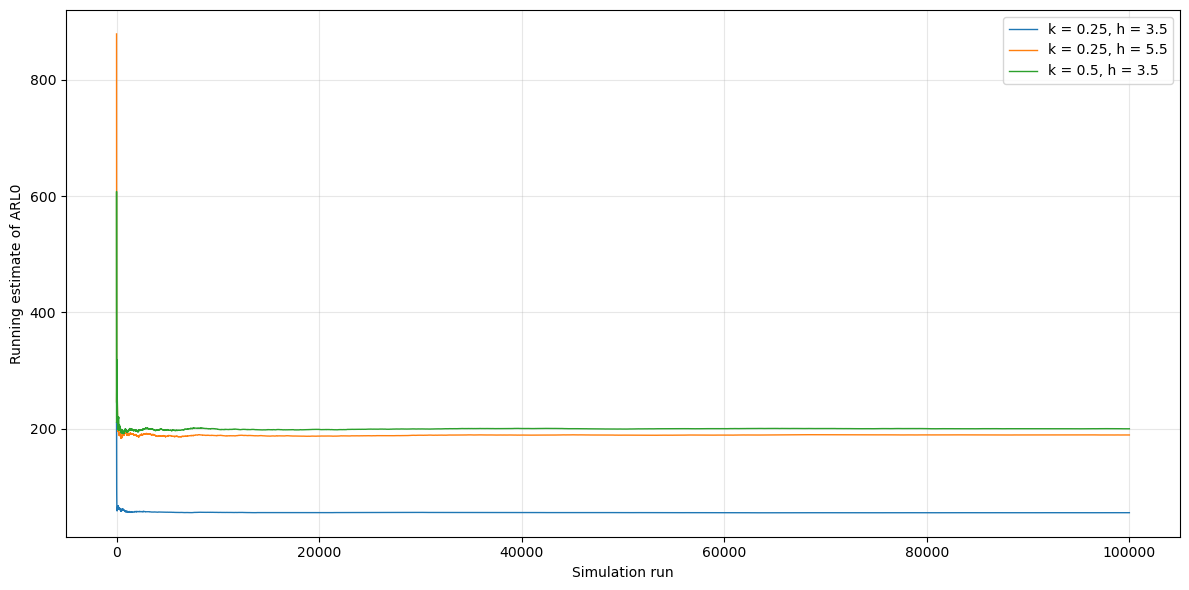
\includegraphics[width=1\textwidth]{4_4ARL.png}
\end{figure}

The simulated results are as follows:
\[
\begin{array}{c|c|c}
k & h & \widehat{ARL}_0 \\ \hline
0.25 & 3.5 & 55.564\\
0.25 & 5.5 & 189.249\\
0.50 & 3.5 & 199.932
\end{array}
\]
\[
\widehat{ARL}_0(0.50,3.5)
>
\widehat{ARL}_0(0.25,5.5)
>
\widehat{ARL}_0(0.25,3.5)
\]

When \(k=0.25\), increasing \(h\) from \(3.5\) to \(5.5\) gives
\[
55.564 \longrightarrow 189.249
\]

Thus,
\[
h\uparrow \quad \Rightarrow \quad ARL_0\uparrow
\]

When \(h=3.5\), increasing \(k\) from \(0.25\) to \(0.5\) gives
\[
55.564 \longrightarrow 199.932
\]

Thus,
\[
k\uparrow \quad \Rightarrow \quad ARL_0\uparrow
\]

Therefore, both larger \(h\) and larger \(k\) make false alarms less frequent under the IC process.

\section*{4.5}
\textbf{Sol.}

For the one-sided upward CUSUM chart (4.7)--(4.8)
\[
C_n^+=\max\{0,C_{n-1}^+ + X_n-k\},
\qquad C_0^+=0
\]

The signal rule is
\[
C_n^+>h
\]

Under the IC process,
\[
X_n\sim N(0,1)
\]

For a given \(h\), define
\[
RL=\min\{n:C_n^+>h\}
\]

Then
\[
\widehat{ARL}_0(h)=\frac{1}{M}\sum_{m=1}^M RL_m
\]

In this problem,
\[
\rho=0.5
\]

We search for \(h\) such that
\[
\left|\widehat{ARL}_0(h)-ARL_0\right|\leq \rho
\]

We calculate it in R:
\begin{codeblock}
\begin{verbatim}
set.seed(611211106)
# Monte Carlo ARL for upward mean CUSUM
simulate_arl_mean_up <- function(k = 0.5, h = 3.5, mu = 0, sd = 1,
                                 M = 5000, Nmax = 10000) {
  rl <- rep(NA_integer_, M)

  for (j in seq_len(M)) {
    cval <- 0

    for (n in seq_len(Nmax)) {
      x <- rnorm(1, mean = mu, sd = sd)
      cval <- max(0, cval + x - k)

      if (cval > h) {
        rl[j] <- n
        break
      }
    }
  }

  mean(rl, na.rm = TRUE)
}

# Bisection search for h using Monte Carlo ARL
search_h_mean_up <- function(target_arl0 = 200, k = 0.5,
                             hL = 0, hU = 15,
                             tol = 0.5, M = 2000,
                             max_iter = 30) {
  history <- data.frame(iter = integer(), h = numeric(), arl = numeric())

  for (iter in seq_len(max_iter)) {
    h <- (hL + hU) / 2
    arl <- simulate_arl_mean_up(k = k, h = h, M = M)

    history <- rbind(
      history,
      data.frame(iter = iter, h = h, arl = arl)
    )

    if (abs(arl - target_arl0) <= tol) break

    if (arl > target_arl0) {
      hU <- h
    } else {
      hL <- h
    }
  }

  list(h = h, arl = arl, history = history)
}
case1 <- search_h_mean_up(target_arl0 = 350, k = 0.25, tol = 0.5)
case2 <- search_h_mean_up(target_arl0 = 350, k = 0.5,  tol = 0.5)
case3 <- search_h_mean_up(target_arl0 = 550, k = 0.5,  tol = 0.5)
\end{verbatim}
\end{codeblock}

The computed results are
\[
\begin{array}{c|c|c|c}
\text{Target } ARL_0 & k & h & \widehat{ARL}_0 \\ \hline
350 & 0.25 & 6.62 & 354.66\\
350 & 0.50 & 4.06 & 349.78\\
550 & 0.50 & 4.47 & 550.36
\end{array}
\]

Therefore, for the same \(ARL_0\), as \(k\) increases, \(h\) decreases;
for the same \(k\), as \(ARL_0\) increases, \(h\) increases.

\section*{4.9}
\textbf{Sol.}

For the two-sided DI-CUSUM chart,
\[
C_n^+=\max\{0,C_{n-1}^+ + X_n-k\},
\qquad C_0^+=0
\]

\[
C_n^-=\min\{0,C_{n-1}^- + X_n+k\},
\qquad C_0^-=0
\]

The signal rule is
\[
C_n^+>h
\quad\text{or}\quad
C_n^-<-h
\]

In this problem,
\[
k=0.5,\qquad h=4.095
\]

For each shifted distribution, define
\[
RL=\min\{n:C_n^+>h \text{ or } C_n^-<-h\}
\]

Using the approximation relationship, if the shifted distribution is
\[
N(\delta,\lambda^2),
\]
then
\[
k^*=\frac{k-|\delta|}{\lambda},
\qquad
h^*=\frac{h}{\lambda}.
\]

Therefore,
\[
ARL_1 \approx
\frac{\exp\{2k^*(h^*+1.166)\}-2k^*(h^*+1.166)-1}
{2(k^*)^2}.
\]

When \(k^*=0\), the limiting value is used:
\[
ARL_1 \approx (h^*+1.166)^2.
\]

We calculate it in R:
\begin{codeblock}
\begin{verbatim}
set.seed(611211106)
# Siegmund approximation for one-sided mean CUSUM ARL0
arl0_siegmund <- function(k, h) {
  if (abs(k) < 1e-12) return(NA_real_)
  a <- h + 1.166
  (exp(2 * k * a) - 2 * k * a - 1) / (2 * k^2)
}

# ARL relationship under N(mu0 + delta, lambda^2 sigma^2)
arl1_from_arl0_approx <- function(k, h, delta = 0, lambda = 1, sigma = 1) {
  k_star <- (k - delta) / (lambda * sigma)
  h_star <- h / (lambda * sigma)

  if (abs(k_star) < 1e-12) return(NA_real_)
  arl0_siegmund(k_star, h_star)
}
k <- 0.5
h <- 4.095

cases <- data.frame(
  case = c("(i)", "(ii)", "(iii)", "(iv)", "(v)", "(vi)"),
  distribution = c("N(0.5,1)", "N(1,1)", "N(-1,1)",
                   "N(0,2^2)", "N(0,0.5^2)", "N(1,2^2)"),
  delta = c(0.5, 1, -1, 0, 0, 1),
  lambda = c(1, 1, 1, 2, 0.5, 2)
)

cases$ARL1 <- mapply(
  arl1_from_arl0_approx,
  k = k,
  h = h,
  delta = cases$delta,
  lambda = cases$lambda
)

cases
\end{verbatim}
\end{codeblock}

The computed results are
\[
\begin{array}{c|c}
\text{Distribution} & \widehat{ARL}_1 \\ \hline
N(0.5,1) & \text{NA} \\
N(1,1) & 8.532 \\
N(-1,1) & 1.589\times 10^6 \\
N(0,2^2) & 1.904\times 10^1 \\
N(0,0.5^2) & 6.691\times 10^7 \\
N(1,2^2) & 6.458
\end{array}
\]

For \(N(0.5,1)\), we have
\[
k^*=\frac{k-\delta}{\lambda}=\frac{0.5-0.5}{1}=0.
\]
Since the Siegmund approximation formula contains \(2(k^*)^2\) in the
denominator, the formula is singular when \(k^*=0\). Therefore, the ARL
value is reported as NA.

From the results, for the same mean shift, a higher variance gives a
lower \(\widehat{ARL}_1\), which makes the control chart more effective.
A negative mean shift or a lower variance gives a larger
\(\widehat{ARL}_1\), which makes the control chart less effective.

Therefore, under the current calculation, this CUSUM design is suitable
for detecting upward mean shifts and variance increases, but not suitable
for detecting downward mean shifts or variance decreases.

\section*{4.19}
\textbf{Sol.}

Let \(X_n\) be the number of junk emails received on day \(n\). Since the $X_n$ are discrete, we use a Poisson CUSUM chart.
The IC mean is $\lambda_0=10$, and the junk email rate has doubled, so the shifted mean is $\lambda_1=20$.
For detecting an upward shift from \(\lambda_0\) to \(\lambda_1\), the reference value is
\[
k^+
=
\frac{\lambda_1-\lambda_0}{\log\lambda_1-\log\lambda_0}
=
\frac{20-10}{\log 20-\log 10}
=
\frac{10}{\log 2}
=
14.427
\]

The upward Poisson CUSUM is
\[
C_n^+=\max\{0,C_{n-1}^+ + X_n-k^+\},
\qquad C_0^+=0
\]

The signal rule is
\[
C_n^+>h^+
\]

The control limit \(h^+\) is chosen so that the IC ARL is approximately 200:
\[
ARL_0\approx 200
\]

Then \(h^+\) is computed in R:
\begin{codeblock}
\begin{verbatim}
set.seed(611211106)

lambda0 <- 10
lambda1 <- 20

k_pois <- (lambda1 - lambda0) /
  (log(lambda1) - log(lambda0))

# Monte Carlo ARL for upward mean CUSUM
simulate_arl_mean_up <- function(k = k_pois, h = 3.5, mu = 0, sd = 1,
                                 M = 5000, Nmax = 10000) {
  rl <- rep(NA_integer_, M)

  for (j in seq_len(M)) {
    cval <- 0

    for (n in seq_len(Nmax)) {
      x <- rpois(1, lambda = lambda0)
      cval <- max(0, cval + x - k)

      if (cval > h) {
        rl[j] <- n
        break
      }
    }
  }

  mean(rl, na.rm = TRUE)
}

# Bisection search for h using Monte Carlo ARL
search_h_mean_up <- function(target_arl0 = 200,
                             hL = 0, hU = 15,
                             tol = 0.5, M = 10000,
                             max_iter = 30) {
  history <- data.frame(iter = integer(), h = numeric(), arl = numeric())

  for (iter in seq_len(max_iter)) {
    h <- (hL + hU) / 2
    arl <- simulate_arl_mean_up(h = h, M = M)

    history <- rbind(
      history,
      data.frame(iter = iter, h = h, arl = arl)
    )

    if (abs(arl - target_arl0) <= tol) break

    if (arl > target_arl0) {
      hU <- h
    } else {
      hL <- h
    }
  }

  list(h = h, arl = arl, history = history)
}
case4 <- search_h_mean_up()
---
> case4[["h"]]
[1] 4.628906
> case4[["arl"]]
[1] 200.425
\end{verbatim}
\end{codeblock}

Under the tolerance \(0.5\), the simulated ARL is close to the target value \(ARL_0=200\). Therefore, the control limit is taken as $$h^+=4.629$$
To find the first signal, we apply the Poisson CUSUM to the observed data in R:
\begin{codeblock}
\begin{verbatim}
# Poisson CUSUM for upward shift in rate
cusum_poisson_up <- function(x, lambda0, lambda1, h = 4.629) {
  k <- (lambda1 - lambda0) / (log(lambda1) - log(lambda0))
  
  C <- numeric(length(x))
  signal <- rep(FALSE, length(x))
  
  for (i in seq_along(x)) {
    previous <- ifelse(i == 1, 0, C[i - 1])
    C[i] <- max(0, previous + x[i] - k)
    signal[i] <- C[i] > h
  }
  
  data.frame(
    n = seq_along(x),
    x = x,
    Cplus = C,
    signal = signal,
    k = k
  )
}

set.seed(611211106)

x_pois <- c(
  14, 10, 6, 10, 9, 7, 17, 9, 13, 10,
  22, 21, 15, 25, 27, 26, 20, 26, 26, 17,
  23, 16, 18, 22, 15, 23, 19, 15, 18, 13
)

pois_df <- cusum_poisson_up(
  x_pois,
  lambda0 = 10,
  lambda1 = 20,
  h = 4.629
)
\end{verbatim}
\end{codeblock}

The result is:
\[
\begin{array}{c|c|c|c}
n & x & C_n^+ & \text{Signal} \\ \hline
1  & 14 & 0.00000 & \text{FALSE} \\
2  & 10 & 0.00000 & \text{FALSE} \\
3  & 6  & 0.00000 & \text{FALSE} \\
4  & 10 & 0.00000 & \text{FALSE} \\
5  & 9  & 0.00000 & \text{FALSE} \\
6  & 7  & 0.00000 & \text{FALSE} \\
7  & 17 & 2.57305 & \text{FALSE} \\
8  & 9  & 0.00000 & \text{FALSE} \\
9  & 13 & 0.00000 & \text{FALSE} \\
10 & 10 & 0.00000 & \text{FALSE} \\
11 & 22 & 7.57305 & \text{TRUE}
\end{array}
\]
\begin{figure}[htbp]
    \centering
    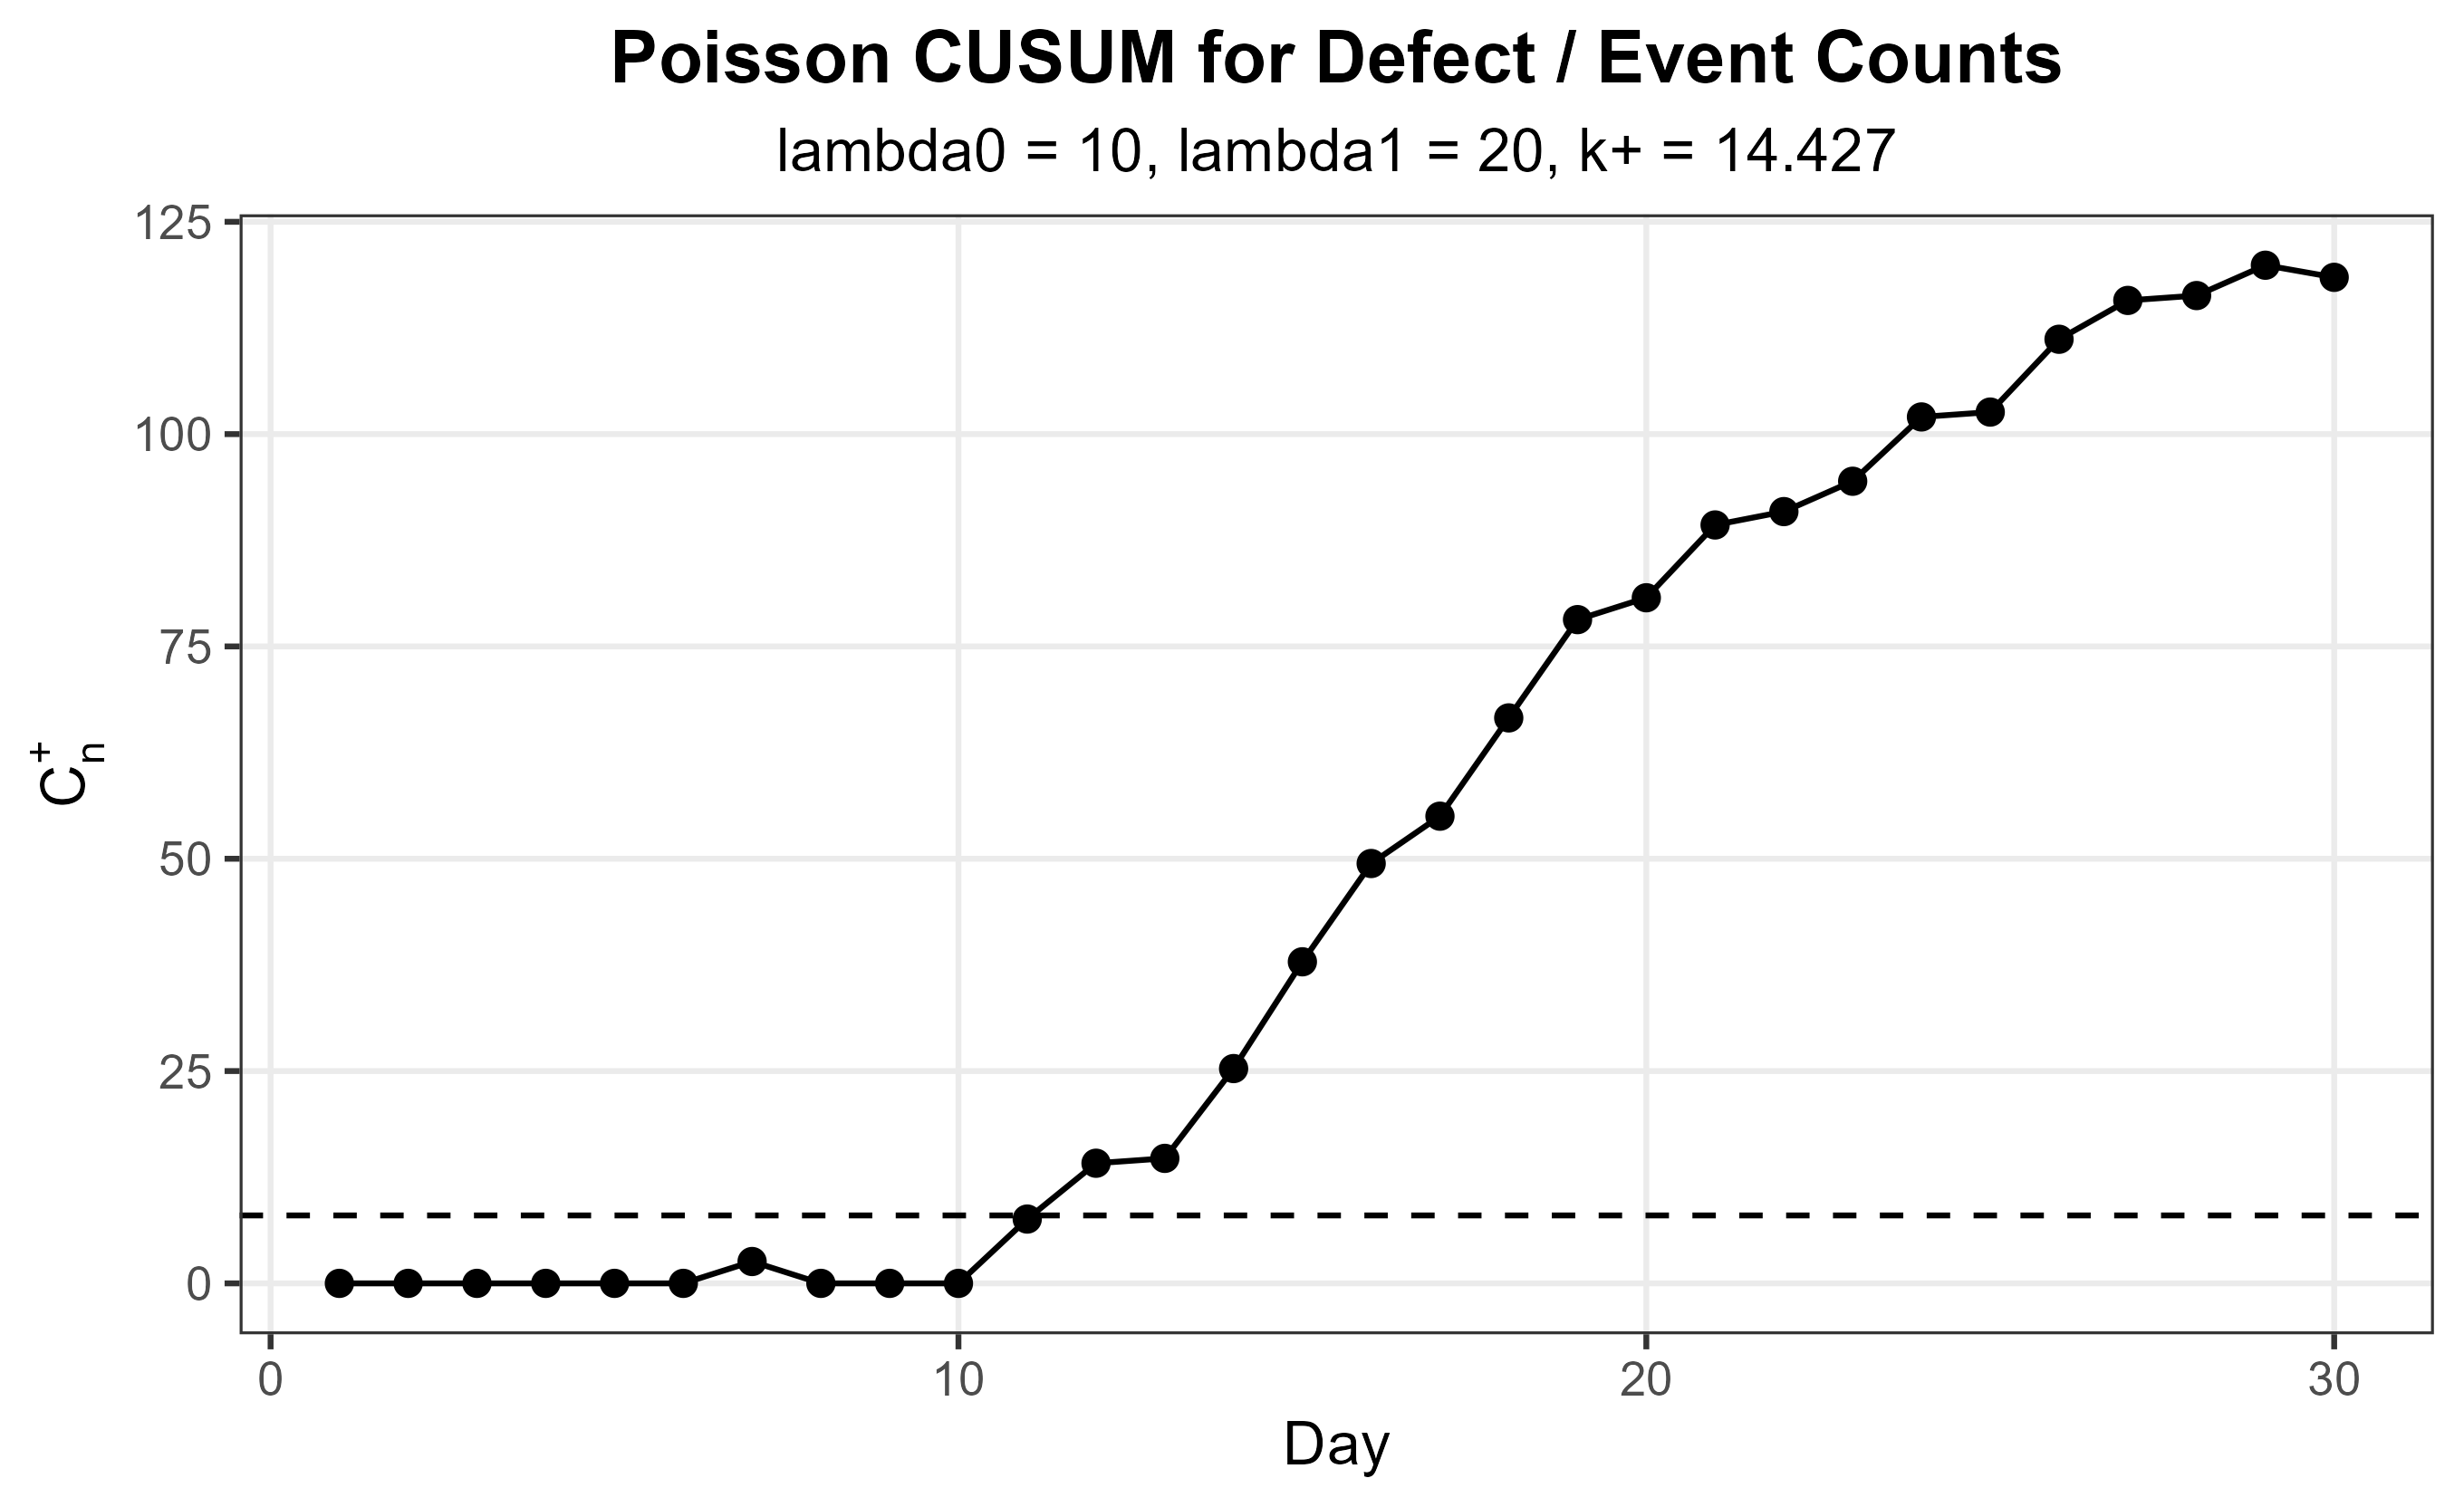
\includegraphics[width=1\textwidth]{4_19.png}
\end{figure}

The first signal occurs at $n=11$ because $C_{11}^+=7.573>4.629=h^+$.
In conclusion, the Poisson CUSUM chart detects an upward shift in the junk email rate at day 11.
\end{document}